\documentclass[10pt]{beamer}

\usetheme[progressbar=frametitle]{metropolis}
\usepackage{appendixnumberbeamer}
\usepackage{subcaption}

\usepackage{booktabs}
\usepackage[scale=2]{ccicons}
\usepackage{svg}

\usepackage{pgfplots}
\usepgfplotslibrary{dateplot}
\usepackage{graphicx}
\usepackage{xspace}
\newcommand{\themename}{\textbf{\textsc{metropolis}}\xspace}
\usepackage{amsmath, amssymb, latexsym}
\usepackage{sidecap}
 \setbeamertemplate{caption}{\raggedright\insertcaption\par}

\usepackage{tikz}
\usetikzlibrary{decorations.pathreplacing}

\title{Persistent homology}
\subtitle{A gentle introduction}
% \date{\today}
\date{}
\author{Daniel Collin}
\setbeamercolor{background canvas}{bg=white}

% \institute{Center for modern beamer themes}
% \titlegraphic{\hfill\includegraphics[height=1.5cm]{logo.pdf}}
\begin{document}
\begin{frame}[fragile]{}
\begin{figure}[ht]
  \centering
  \begin{subfigure}[t]{.5\linewidth}
    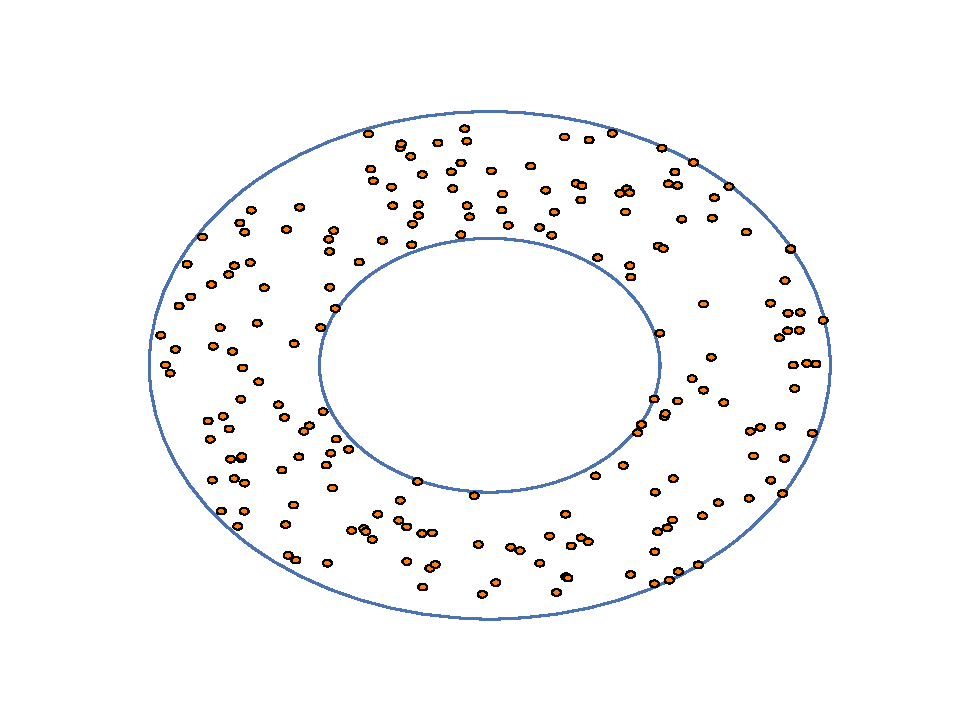
\includegraphics[scale=.35]{annulus.pdf}
    \caption{\label{annulus:points}}
 \end{subfigure}%
  \begin{subfigure}[t]{.5\linewidth}
    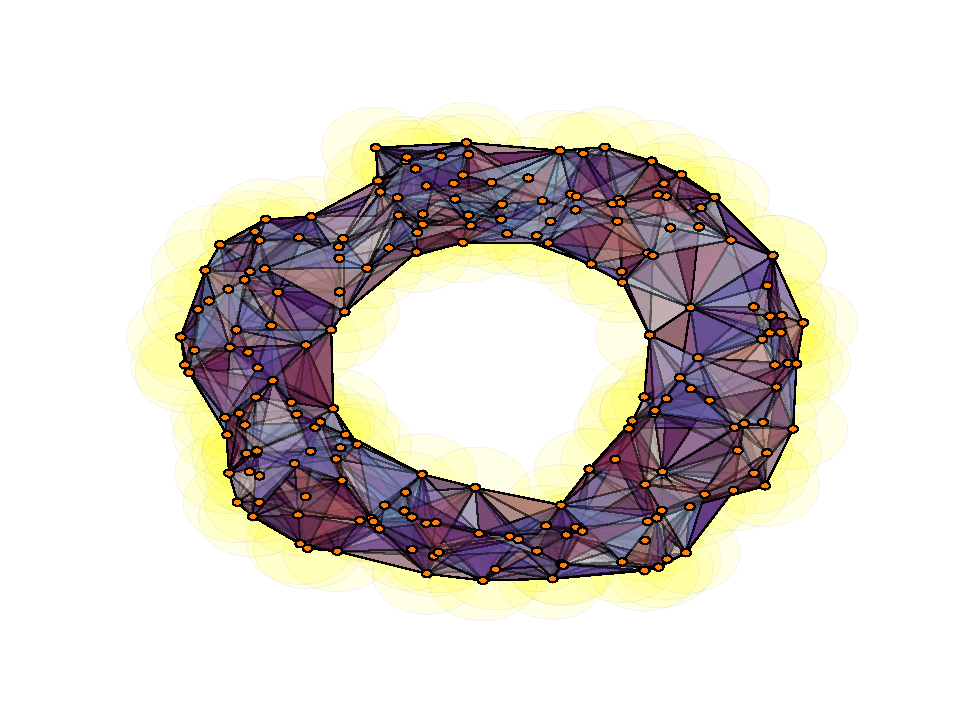
\includegraphics[scale=.35]{annulus_rips.pdf}
    \caption{\label{annulus:imposed}}
 \end{subfigure}
\end{figure}

\end{frame}

\begin{frame}[fragile]{}
\begin{figure}
  \centering
  \begin{subfigure}[t]{.5\linewidth}
    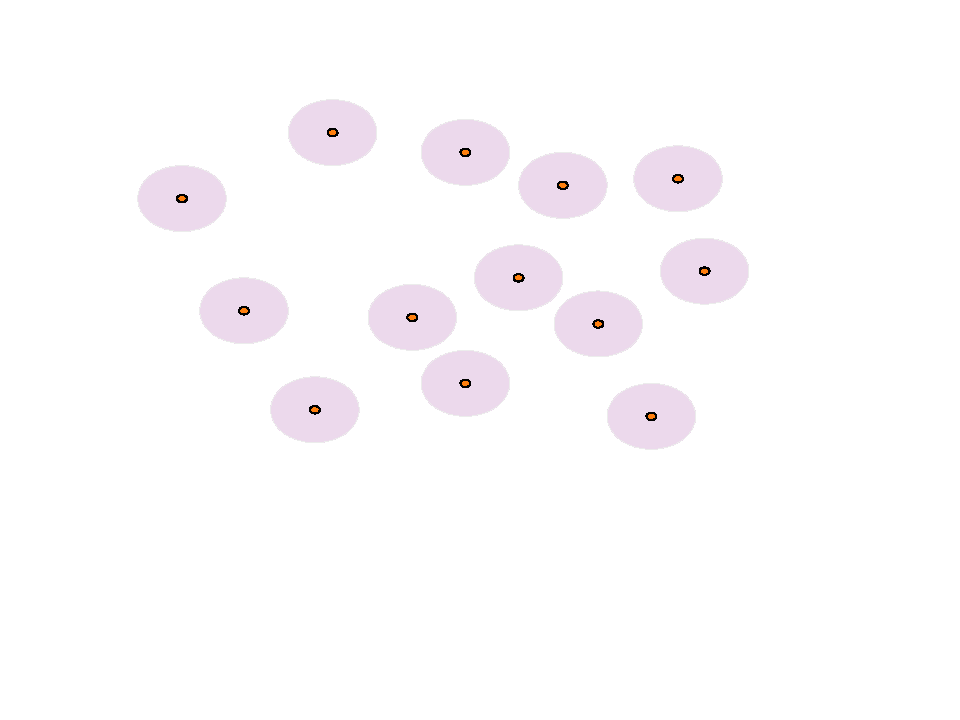
\includegraphics[scale=.4]{rips_eps=01.pdf}
    \caption{$\epsilon=0.1$}
 \end{subfigure}%
  \begin{subfigure}[t]{.5\linewidth}
    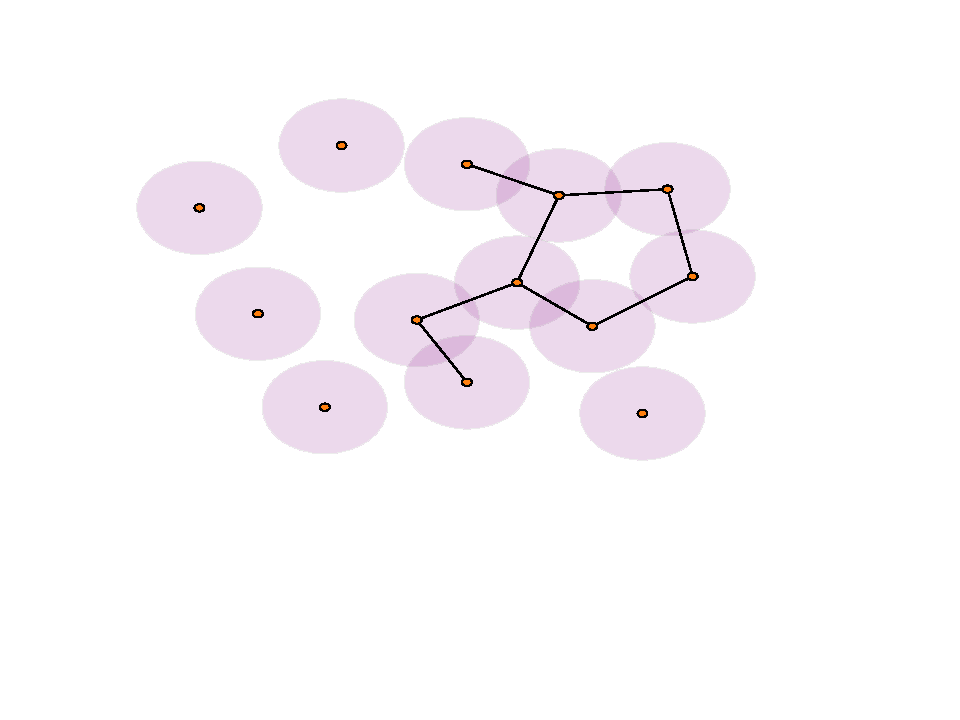
\includegraphics[scale=.4]{rips_eps=015.pdf}
    \caption{$\epsilon=0.15$}
 \end{subfigure}
  \begin{subfigure}[b]{.49\linewidth}
    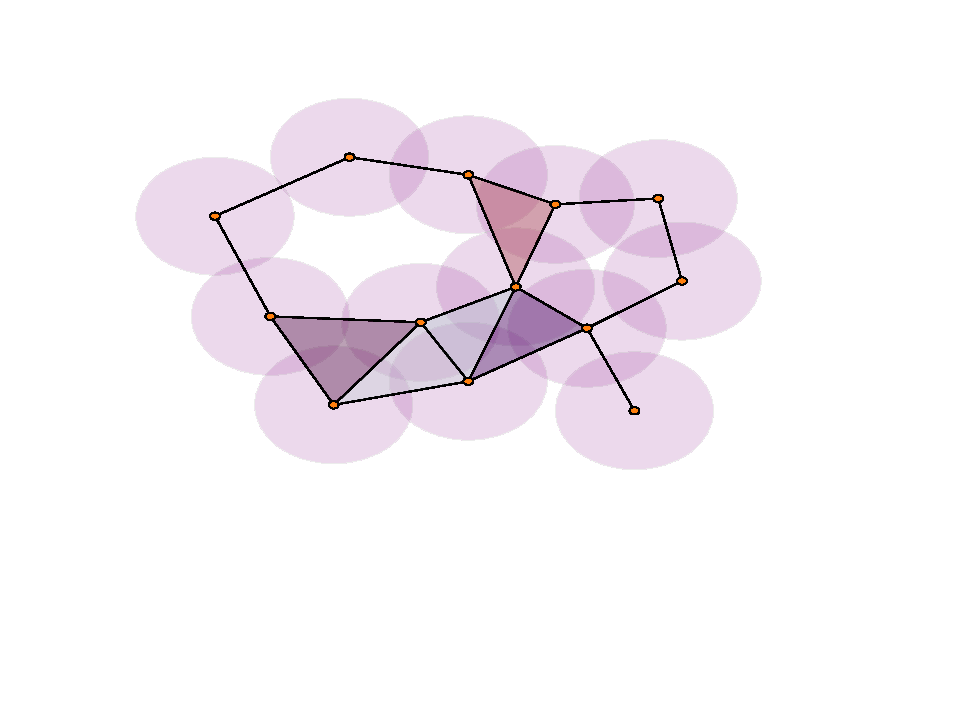
\includegraphics[scale=.4]{rips_eps=02.pdf}
    \caption{$\epsilon=0.2$}
 \end{subfigure}
  \begin{subfigure}[b]{.5\linewidth}
    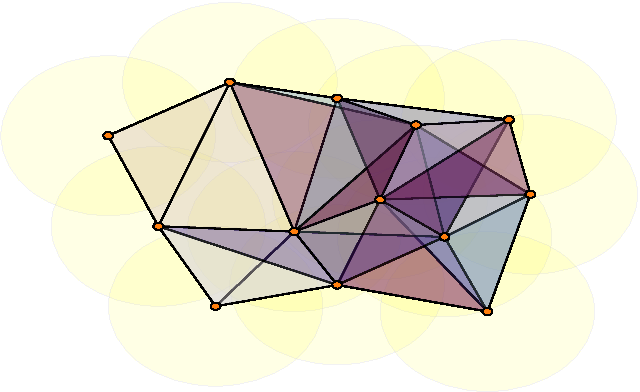
\includegraphics[scale=.4]{rips_eps=03.pdf}
    \caption{$\epsilon=0.3$}
 \end{subfigure}
\end{figure}
\end{frame}

\begin{frame}[fragile]{}
\begin{figure}
  \centering
  \scalebox{0.7}{
\begin{tikzpicture}
\node[inner sep=0pt] (barcode) at (0,0)
    {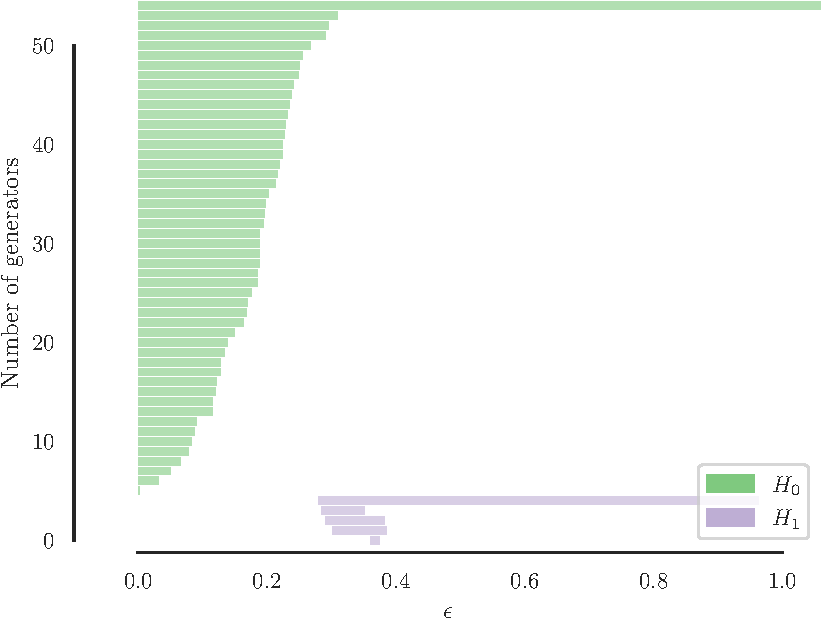
\includegraphics[scale=0.7]{barcode.pdf}};

\node[draw=black!100,line width=0.6mm, inner sep=0pt] (annulus0) at (-3.2,5.1)
    {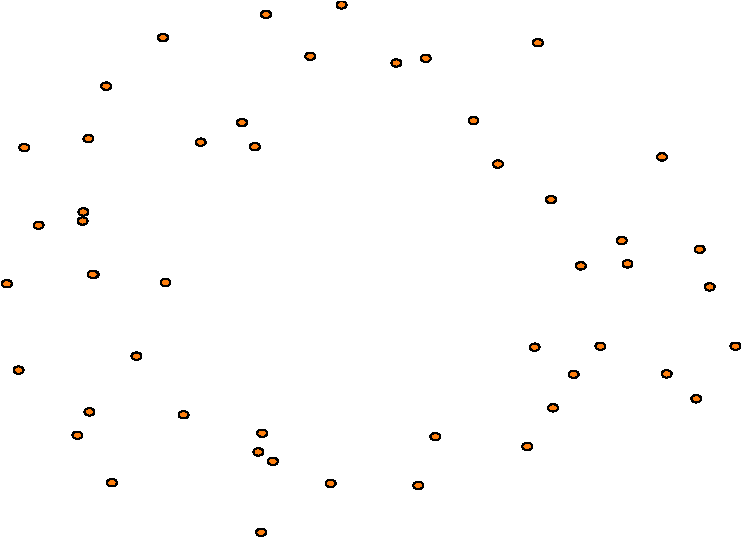
\includegraphics[scale=0.3]{annulus_eps0.pdf}};
    \draw[dotted,thick] (annulus0.south) -- (-3.2,-2.9);

\node[draw=black!100,line width=0.6mm, inner sep=0pt] (annulus3) at (-1,8)
    {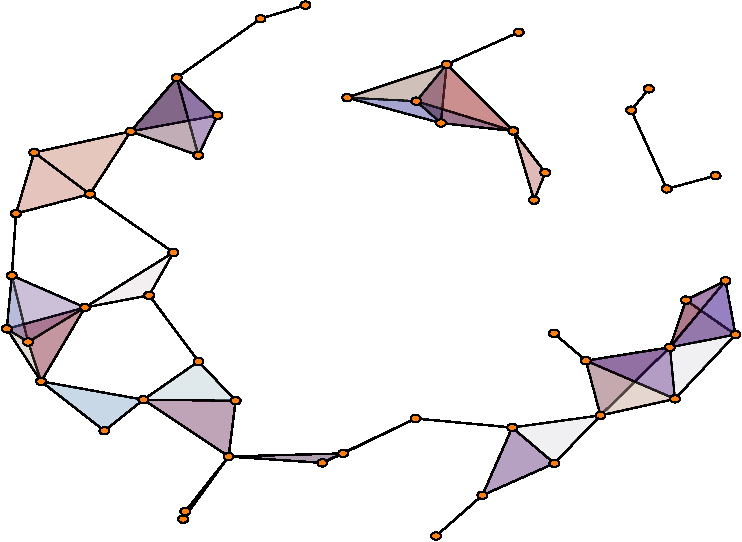
\includegraphics[scale=0.3]{annulus_eps3.pdf}};
\draw[dotted,thick] (annulus3.south) -- (-1,-2.9);

\node[draw=black!100,line width=0.6mm, inner sep=0pt] (annulus5) at (1.2,5.1)
    {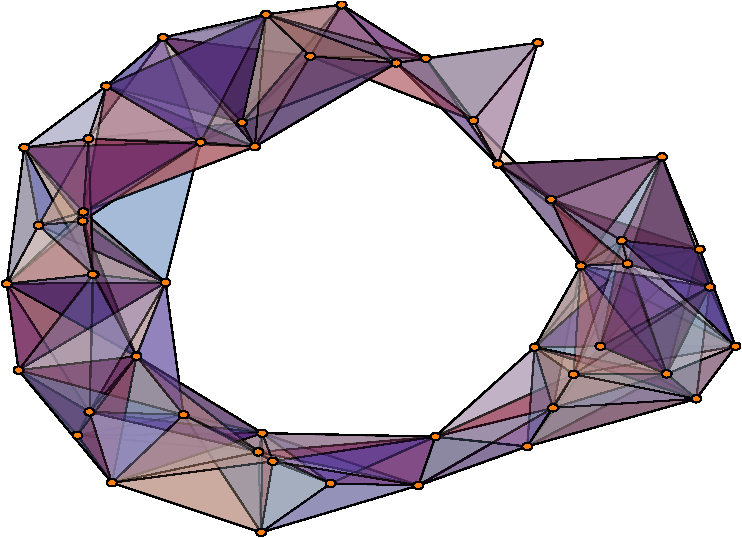
\includegraphics[scale=0.3]{annulus_eps5.pdf}};
    \draw[dotted,thick] (annulus5.south) -- (1.2,-2.9);
\node[draw=black!100,line width=0.6mm, inner sep=0pt] (annulus10) at (4.4,8)
    {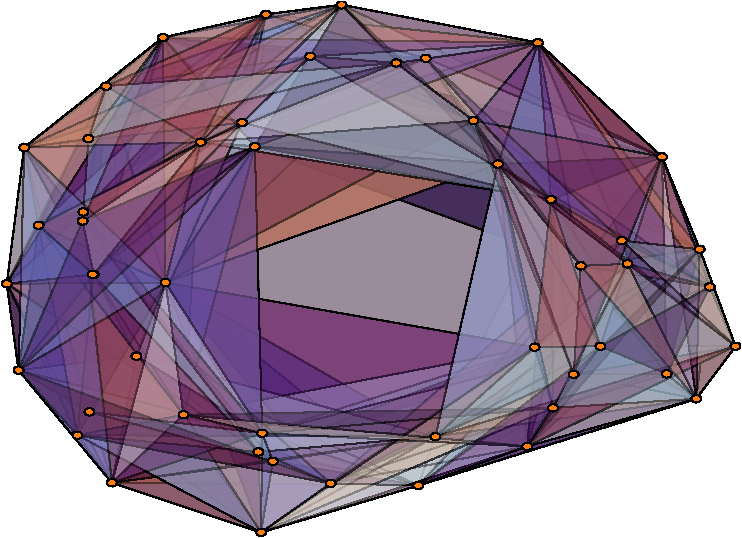
\includegraphics[scale=0.3]{annulus_eps10.pdf}};
\draw[dotted,thick] (annulus10.south) -- (4.4,-1.8);
\draw[dotted,thick] (4.4,-2.74) -- (4.4,-2.9);
\end{tikzpicture}
}
\end{figure}
\end{frame}

\begin{frame}[fragile]{}

  \begin{figure}[ht]
    \centering
    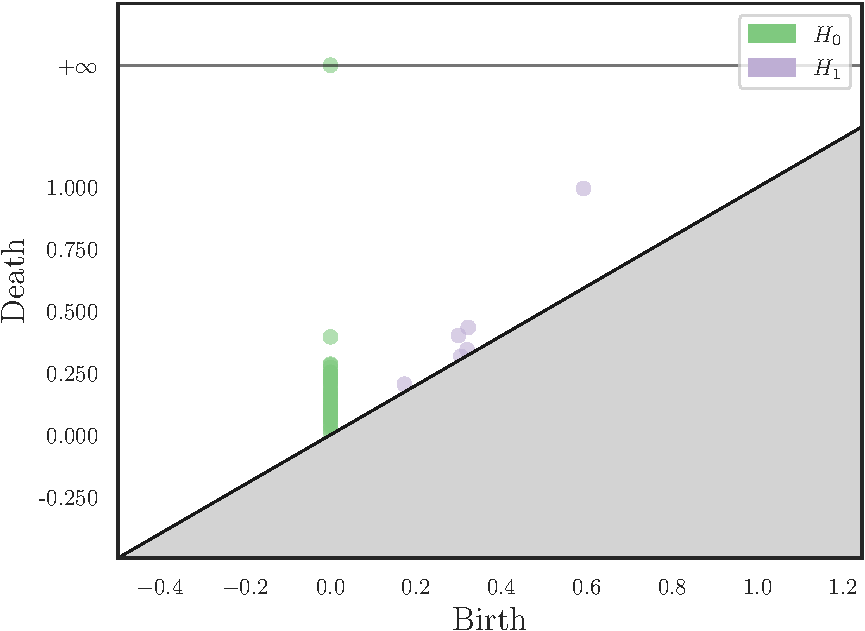
\includegraphics[scale=0.7]{diagram.pdf}
  \end{figure}
\end{frame}

\begin{frame}[fragile]{}
\begin{figure}[ht]
  \centering
  \begin{subfigure}{.5 \linewidth}
    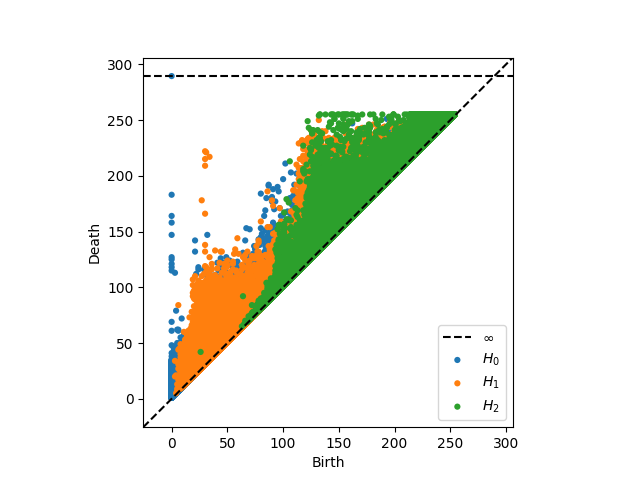
\includegraphics[scale=0.3]{persistence_diagrams/60185_multi_ph.png}
    \caption{60185}
  \end{subfigure}%
  \begin{subfigure}{.5 \linewidth}
    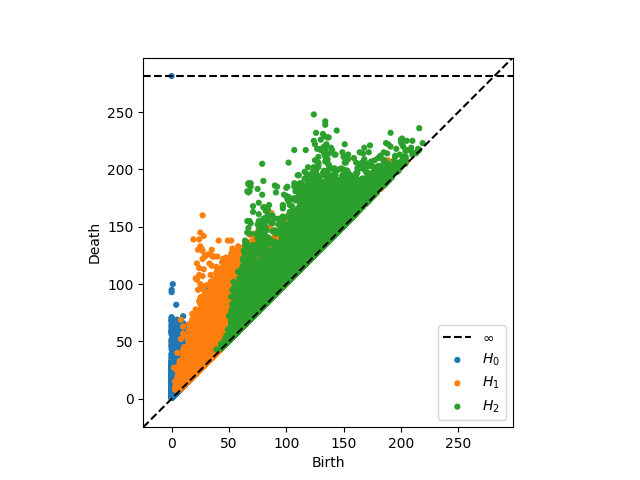
\includegraphics[scale=0.3]{persistence_diagrams/60186_multi_ph.png}
    \caption{60186}
  \end{subfigure}
  \begin{subfigure}{.5 \linewidth}
    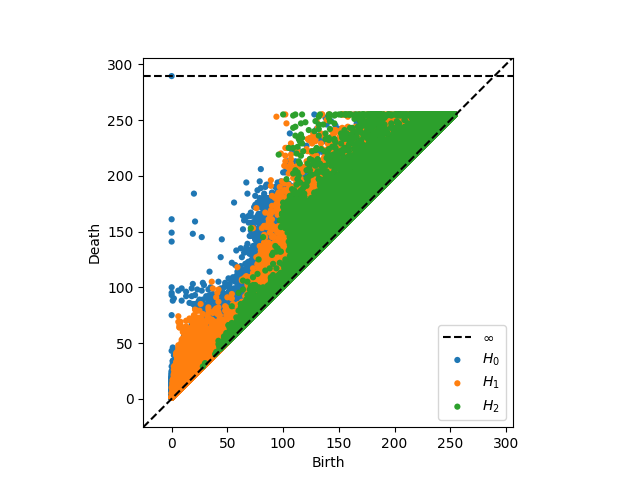
\includegraphics[scale=0.3]{persistence_diagrams/77066_multi_ph.png}
    \caption{77066}
  \end{subfigure}%
  \begin{subfigure}{.5 \linewidth}
    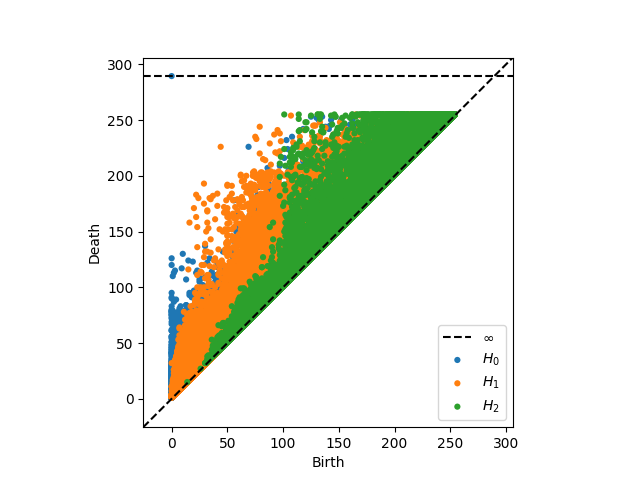
\includegraphics[scale=0.3]{persistence_diagrams/77967_multi_ph.png}
    \caption{77967}
  \end{subfigure}
\end{figure}
\end{frame}

\begin{frame}[fragile]{}
\begin{figure}[ht]
  \centering
  \begin{subfigure}{.5 \linewidth}
    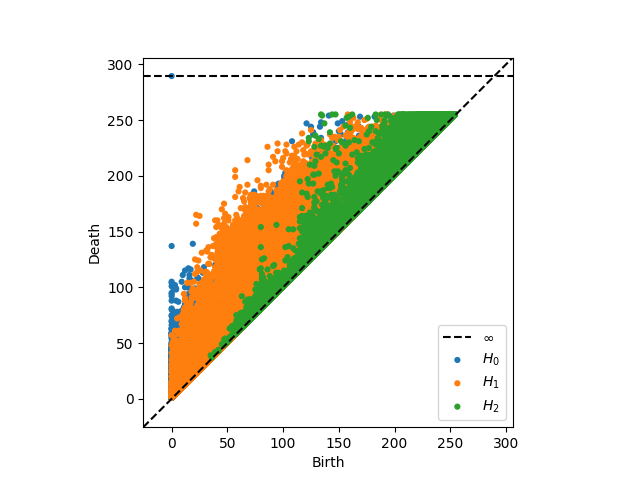
\includegraphics[scale=0.3]{persistence_diagrams/77970_multi_ph.png}
    \caption{77970}
  \end{subfigure}%
  \begin{subfigure}{.5 \linewidth}
    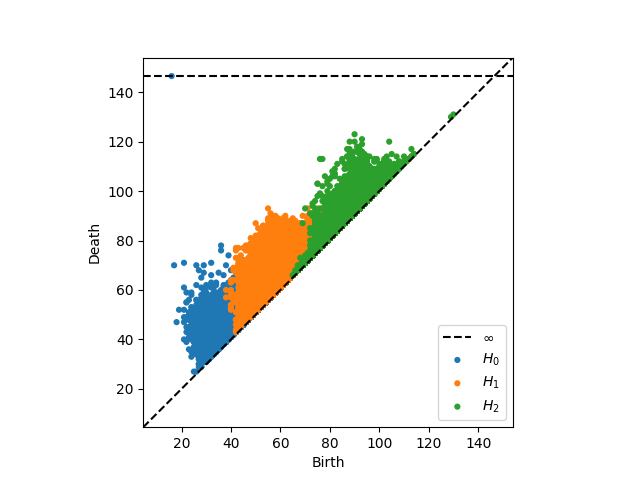
\includegraphics[scale=0.3]{persistence_diagrams/77971_multi_ph.png}
    \caption{77971}
  \end{subfigure}
  \begin{subfigure}{.5 \linewidth}
    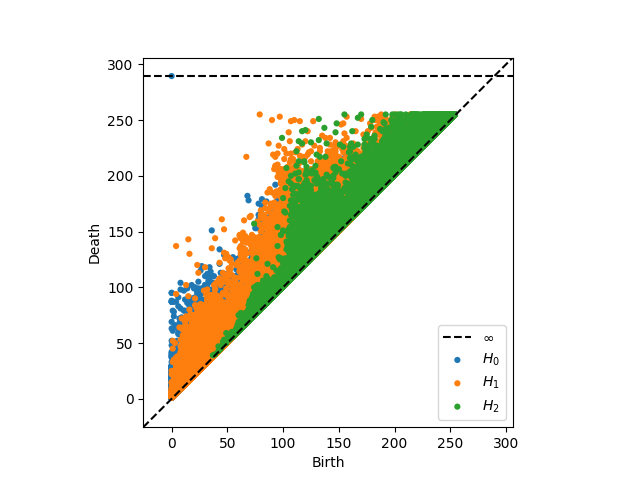
\includegraphics[scale=0.3]{persistence_diagrams/77973_multi_ph.png}
    \caption{77973}
  \end{subfigure}%
  \begin{subfigure}{.5 \linewidth}
    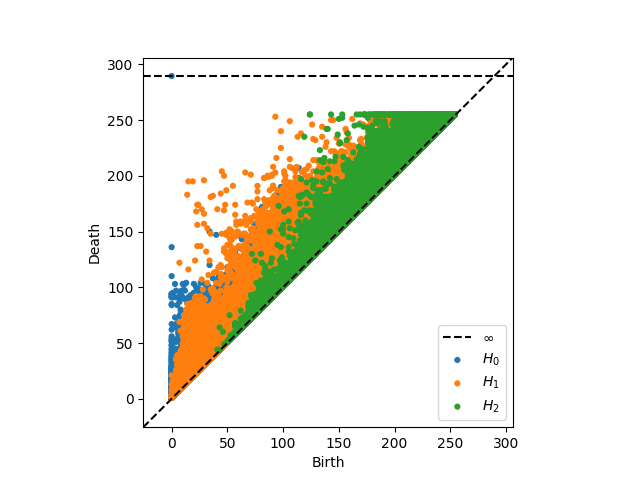
\includegraphics[scale=0.3]{persistence_diagrams/77974_multi_ph.png}
    \caption{77974}
  \end{subfigure}
\end{figure}
\end{frame}
\begin{frame}[fragile]{}
\begin{figure}[ht]
  \centering
  \begin{subfigure}{.33 \linewidth}
    \fbox{
      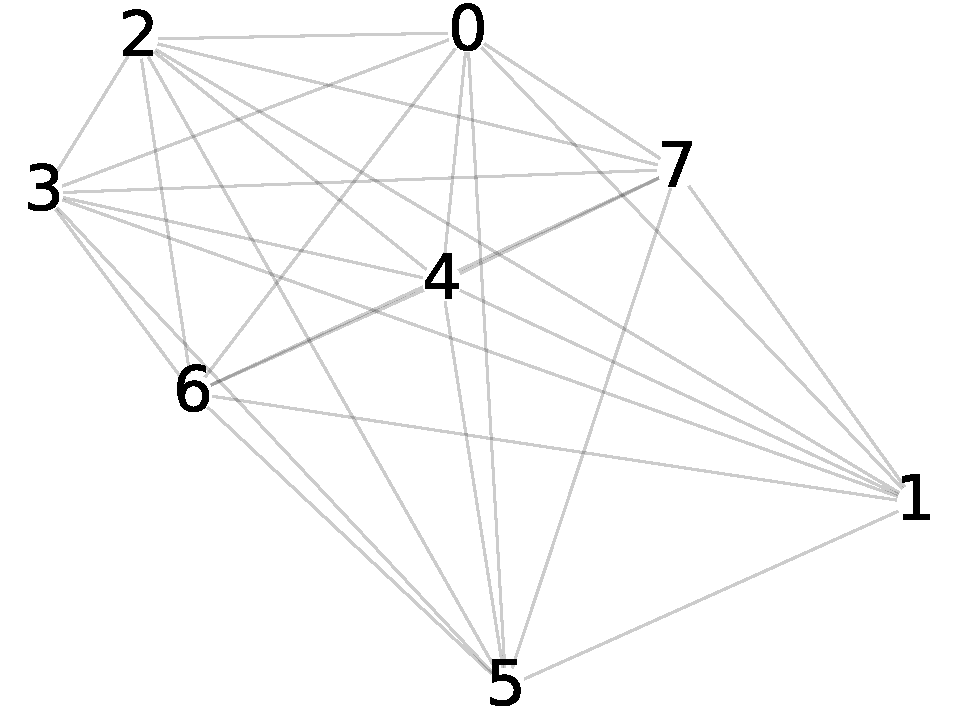
\includegraphics[scale=0.15]{persistence_diagrams/distances/graphs/bottleneck_h0_graph.pdf}
      }
  \end{subfigure}%
  \begin{subfigure}{.33 \linewidth}
    \fbox{
      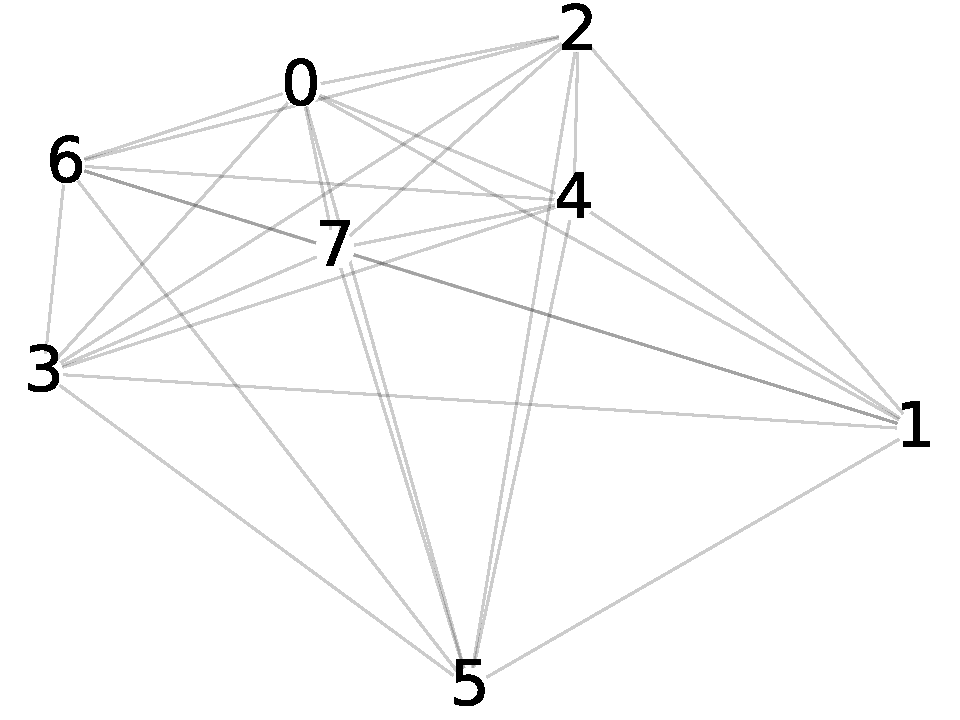
\includegraphics[scale=0.15]{persistence_diagrams/distances/graphs/bottleneck_h1_graph.pdf}
      }
  \end{subfigure}%
  \begin{subfigure}{.33 \linewidth}
    \fbox{
    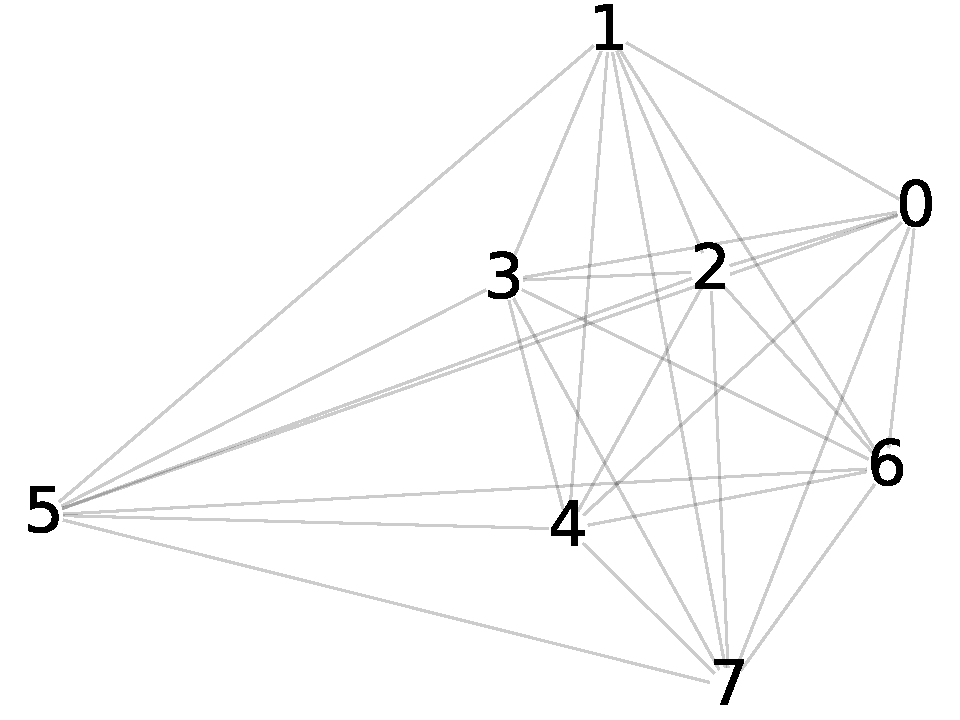
\includegraphics[scale=0.15]{persistence_diagrams/distances/graphs/bottleneck_h2_graph.pdf}
    }
  \end{subfigure}

  \begin{subfigure}{.33 \linewidth}
    \fbox{
    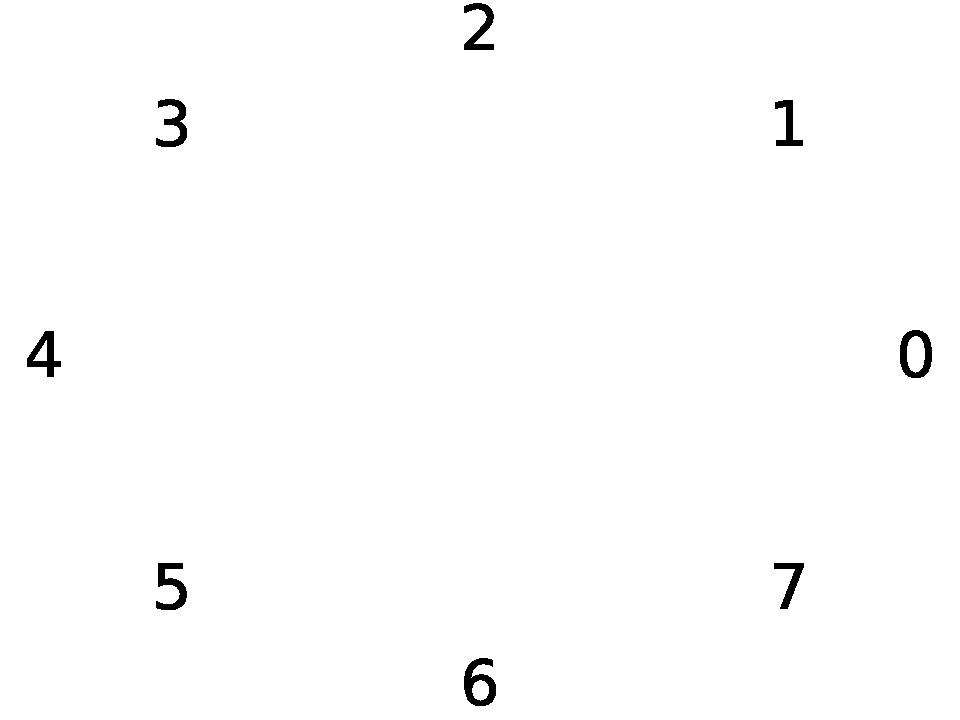
\includegraphics[scale=0.15]{persistence_diagrams/distances/graphs/wasserstein_h0_graph.pdf}
    }
  \end{subfigure}%
  \begin{subfigure}{.33 \linewidth}
    \fbox{
    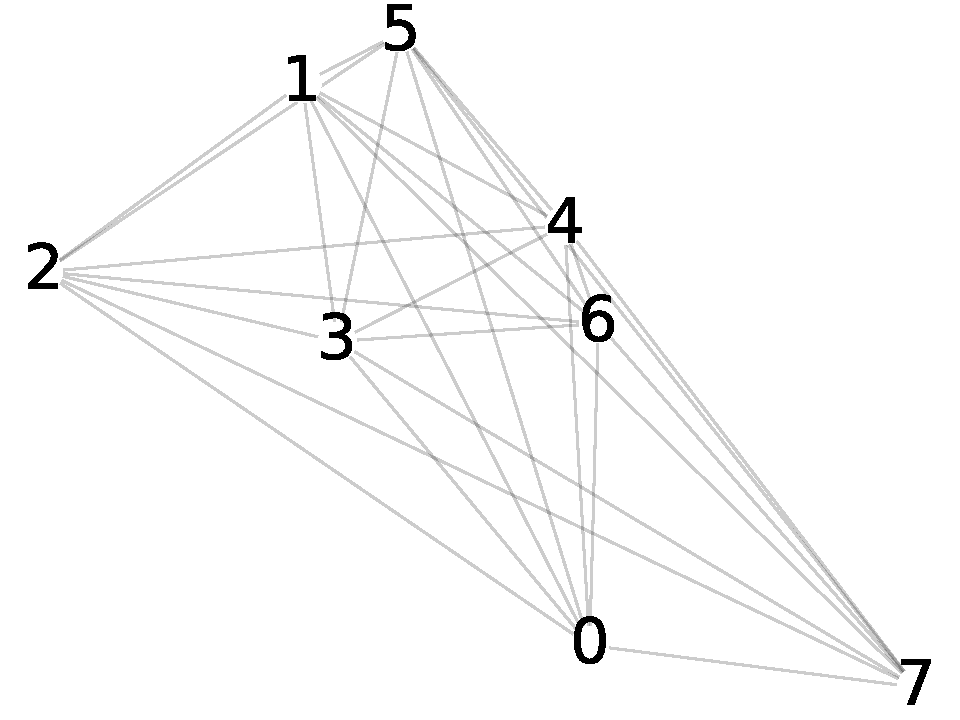
\includegraphics[scale=0.15]{persistence_diagrams/distances/graphs/wasserstein_h1_graph.pdf}
    }
  \end{subfigure}%
  \begin{subfigure}{.33 \linewidth}
    \fbox{
    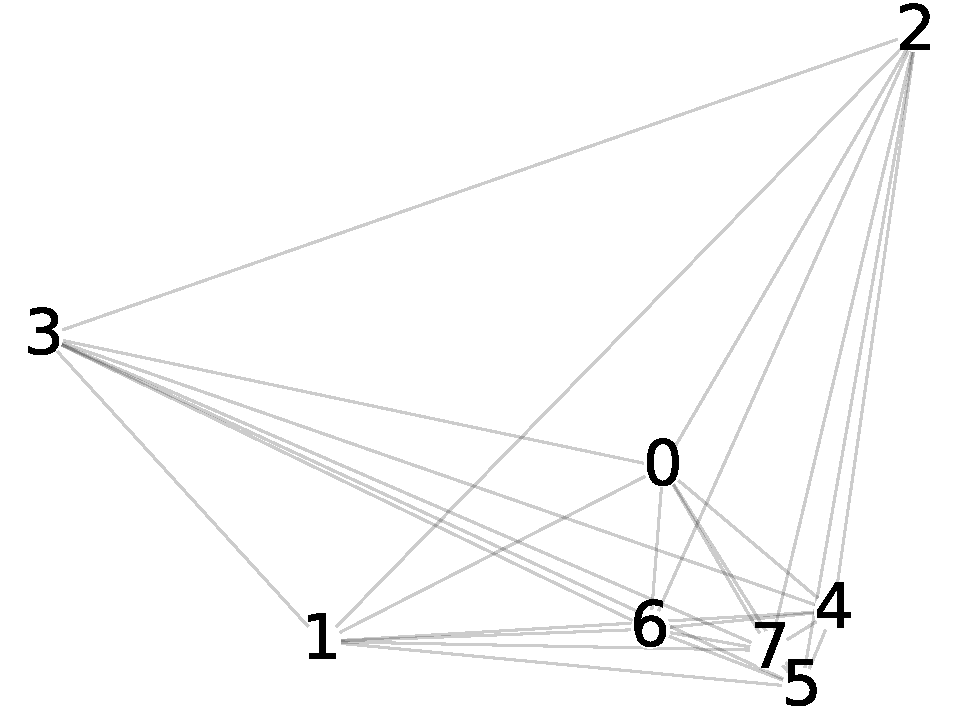
\includegraphics[scale=0.15]{persistence_diagrams/distances/graphs/wasserstein_h2_graph.pdf}
    }
  \end{subfigure}%
\end{figure}
\end{frame}

\begin{frame}[fragile]{}

\begin{figure}[ht]
  \centering
  \begin{subfigure}{.32 \linewidth}
    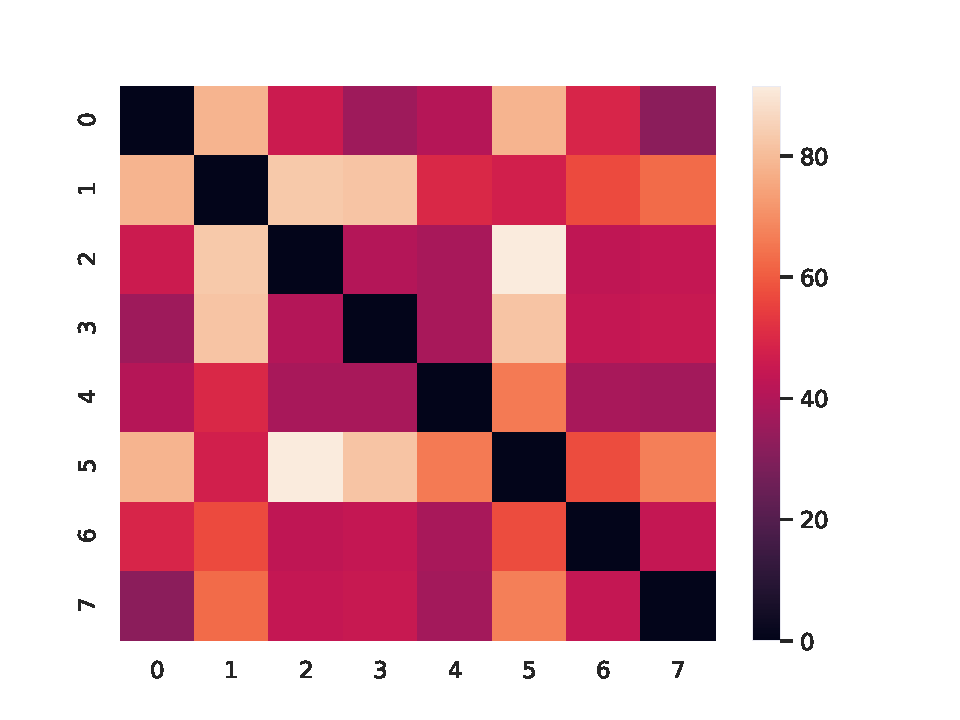
\includegraphics[scale=0.2]{persistence_diagrams/distances/heatmaps/bottleneck_h0.npy.pdf}
  \end{subfigure}%
  \begin{subfigure}{.32 \linewidth}
    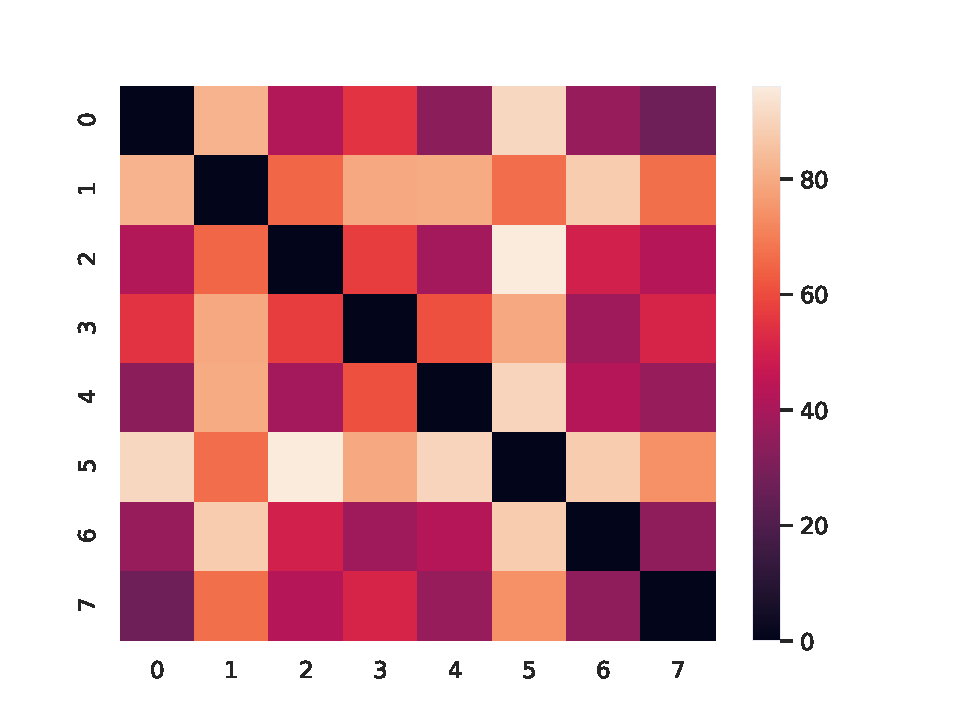
\includegraphics[scale=0.2]{persistence_diagrams/distances/heatmaps/bottleneck_h1.npy.pdf}
  \end{subfigure}%
  \begin{subfigure}{.32 \linewidth}
    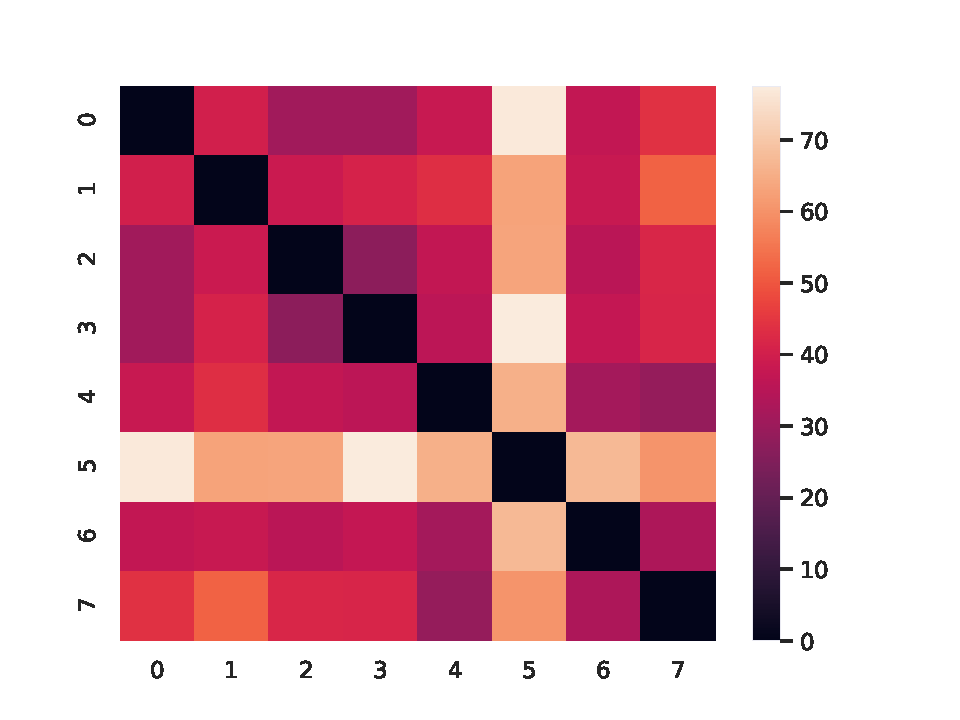
\includegraphics[scale=0.2]{persistence_diagrams/distances/heatmaps/bottleneck_h2.npy.pdf}
  \end{subfigure}

  \begin{subfigure}{.32 \linewidth}
    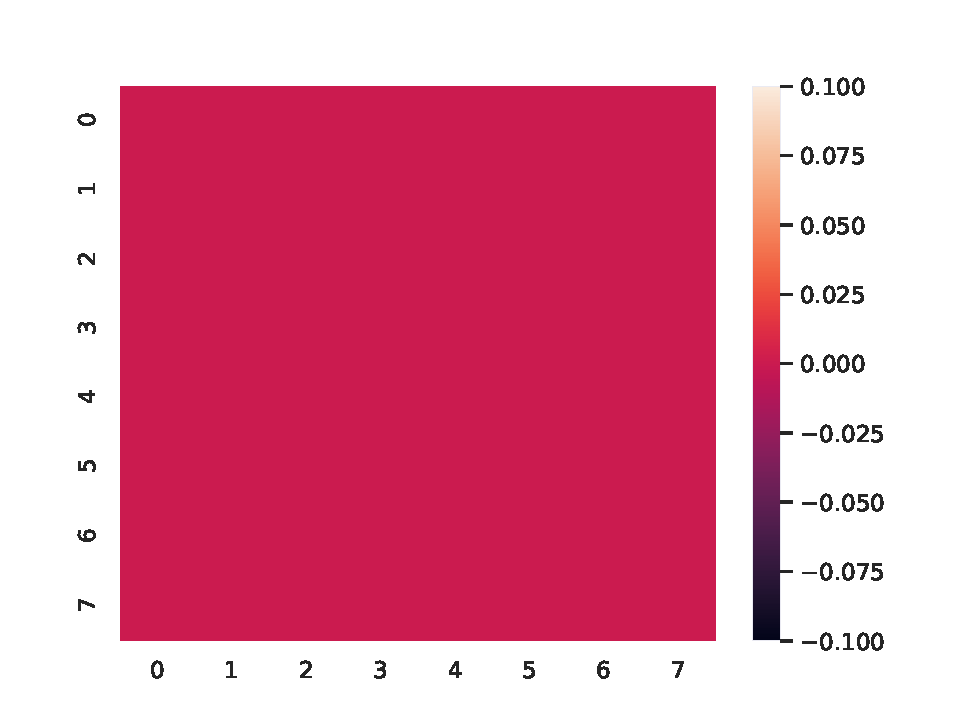
\includegraphics[scale=0.2]{persistence_diagrams/distances/heatmaps/wasserstein_h0.npy.pdf}
  \end{subfigure}%
  \begin{subfigure}{.32 \linewidth}
    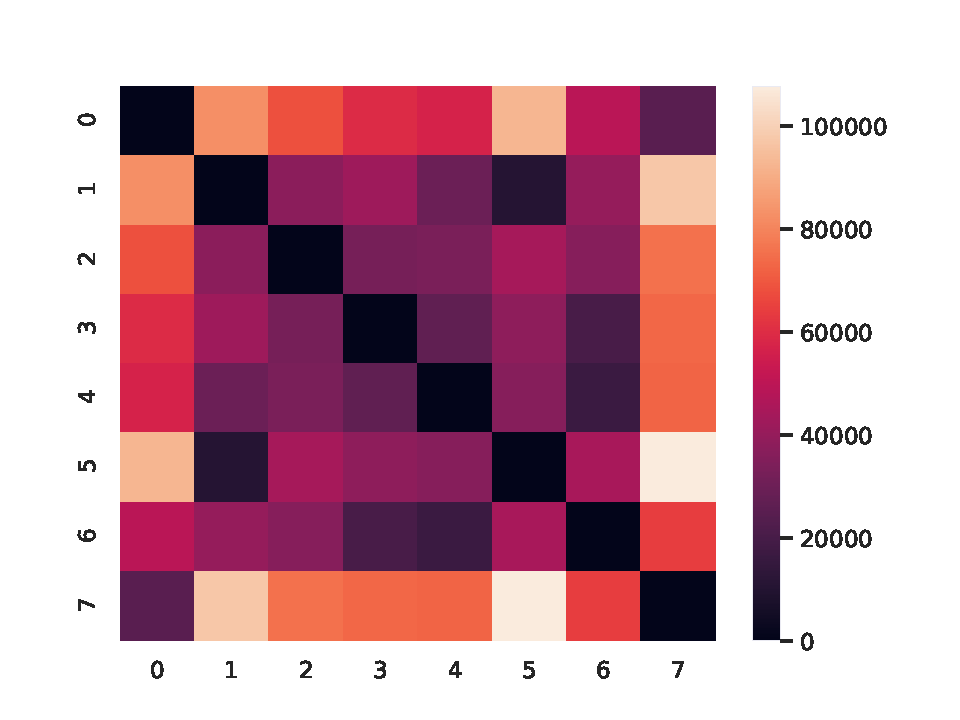
\includegraphics[scale=0.2]{persistence_diagrams/distances/heatmaps/wasserstein_h1.npy.pdf}
  \end{subfigure}%
  \begin{subfigure}{.32 \linewidth}
    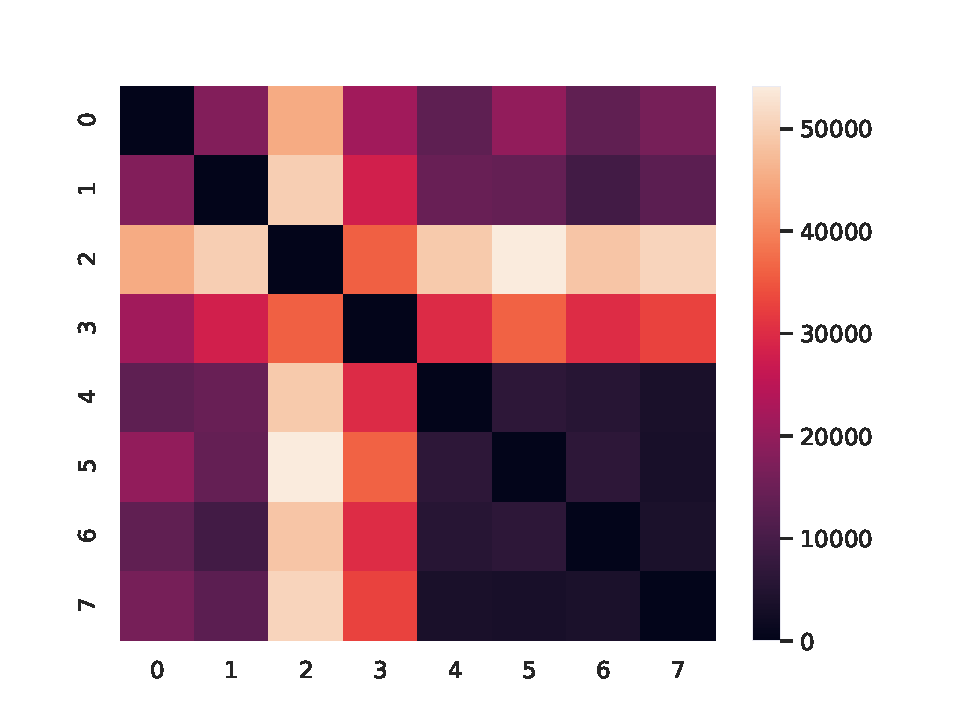
\includegraphics[scale=0.2]{persistence_diagrams/distances/heatmaps/wasserstein_h2.npy.pdf}
  \end{subfigure}%
\end{figure}
\end{frame}
\end{document}
